% Options for packages loaded elsewhere
\PassOptionsToPackage{unicode}{hyperref}
\PassOptionsToPackage{hyphens}{url}
\documentclass[
  journal]{IEEEtran}
\usepackage{xcolor}
\usepackage{amsmath,amssymb}
\setcounter{secnumdepth}{5}
\usepackage{iftex}
\ifPDFTeX
  \usepackage[T1]{fontenc}
  \usepackage[utf8]{inputenc}
  \usepackage{textcomp} % provide euro and other symbols
\else % if luatex or xetex
  \usepackage{unicode-math} % this also loads fontspec
  \defaultfontfeatures{Scale=MatchLowercase}
  \defaultfontfeatures[\rmfamily]{Ligatures=TeX,Scale=1}
\fi
\usepackage{lmodern}
\ifPDFTeX\else
  % xetex/luatex font selection
  \setmainfont[]{Times New Roman}
  \setmathfont[]{STIX Two Math}
\fi
% Use upquote if available, for straight quotes in verbatim environments
\IfFileExists{upquote.sty}{\usepackage{upquote}}{}
\IfFileExists{microtype.sty}{% use microtype if available
  \usepackage[]{microtype}
  \UseMicrotypeSet[protrusion]{basicmath} % disable protrusion for tt fonts
}{}
\makeatletter
\@ifundefined{KOMAClassName}{% if non-KOMA class
  \IfFileExists{parskip.sty}{%
    \usepackage{parskip}
  }{% else
    \setlength{\parindent}{0pt}
    \setlength{\parskip}{6pt plus 2pt minus 1pt}}
}{% if KOMA class
  \KOMAoptions{parskip=half}}
\makeatother
\setlength{\emergencystretch}{3em} % prevent overfull lines
\providecommand{\tightlist}{%
  \setlength{\itemsep}{0pt}\setlength{\parskip}{0pt}}
\usepackage{graphicx}
\usepackage{bookmark}
\IfFileExists{xurl.sty}{\usepackage{xurl}}{} % add URL line breaks if available
\urlstyle{same}
\hypersetup{
  pdftitle={LinDistFlow-Quantile Screen: A Baseline Heuristic for Distribution Voltage-Risk Filtering},
  pdfauthor={Siqiang Zhao (corresponding author); Fengxiang Zhang},
  hidelinks,
  pdfcreator={LaTeX via pandoc}}

\title{LinDistFlow-Quantile Screen: A Baseline Heuristic for
Distribution Voltage-Risk Filtering}
\author{Siqiang Zhao (corresponding author) \and Fengxiang Zhang}
\date{Generated 2026-07-03 02:31 UTC}

\begin{document}
\maketitle

Siqiang Zhao, Sichuan University-Pittsburgh Institute, Chengdu, China,
2023141520257@stu.scu.edu.cn; Fengxiang Zhang, Southwest Jiaotong
University, Chengdu, China, zfengxiang309@gmail.com.

\textbf{Corresponding author:} Siqiang Zhao,
2023141520257@stu.scu.edu.cn.

\section*{Abstract}\label{abstract}
\addcontentsline{toc}{section}{Abstract}

This paper defines a minimal voltage-risk filtering baseline for
distribution feeders. The baseline intentionally uses only two
transparent components: a squared-voltage LinDistFlow proxy computed
from pre-dispatch net-injection forecasts and one global empirical
quantile computed on a calibration split. It contains no residual
learner, no topology/PV/loading conditioned calibration, and no graph
model. The purpose is not to outperform learned screening methods, but
to provide a reproducible lower-complexity reference that exposes what a
purely physical proxy plus a pooled uncertainty radius can and cannot
do. On IEEE 33-bus and 69-bus feeder scenarios, the LinDistFlow-only
screen gives 0.00140 p.u. RMSE, 0.91356 empirical bus-level coverage,
and 0.00474 p.u. mean interval width in the representative random split.
Across three random seeds, the global-quantile screen preserves
scenario-level recall in the tested split family while using
substantially wider intervals than learned residual screens. The
contribution is a baseline implementation note with a precise operating
boundary, not an AC feasibility certificate, an optimization controller,
or a reduced version of a learned screening method.

\section*{Index Terms}\label{index-terms}
\addcontentsline{toc}{section}{Index Terms}

LinDistFlow; Quantile calibration; Voltage risk; Distribution feeders;
Screening baseline

\section{Introduction}\label{introduction}

Distribution operators and researchers often need a quick reference
method for deciding whether forecasted operating scenarios deserve
detailed AC analysis. LinDistFlow-style approximations are attractive
for this role because they are interpretable, inexpensive, and directly
tied to feeder topology and branch impedances. Their weakness is equally
clear: they ignore losses, phase imbalance, nonlinear AC effects, and
local model errors that can become important near voltage limits.

This note asks a deliberately narrow question: how far can one get with
a LinDistFlow voltage proxy and a single global empirical error radius?
The answer is useful because it gives later methods a clean baseline.
Distribution voltage-screening papers often compare against different
point predictors, different voltage margins, or unpublished engineering
heuristics. A transparent baseline with fixed equations, split protocol,
and reported screening metrics helps make future comparisons less
dependent on ad hoc strawmen.

The paper is therefore written as an implementation note. It reports the
inputs, equations, split protocol, and measured behavior of the
LinDistFlow global-quantile screen. It does not introduce residual
learning, conditioned conformal calibration, topology-aware feature
learning, or DMS control logic. Those topics belong to separate method
or system-integration papers.

This paper is the baseline companion to two related studies. The
VoltGuard method paper studies physics-informed topology-aware residual
learning with conditioned conformal calibration. The DMS integration
paper studies how a calibrated screen should be embedded into release,
watch, and corrective-audit queues. This note supplies the minimal
reference screen that both papers and future work can use as a common
lower-complexity comparator.

\subsection{Related Baseline Practice and
Positioning}\label{related-baseline-practice-and-positioning}

Voltage-screening papers use several kinds of lower-complexity
comparisons. Some use static voltage margins or flat nominal-voltage
assumptions; these are easy to reproduce but ignore feeder impedance and
downstream power flow. Some use historical bus envelopes; these can be
conservative when the history is rich, but they do not extrapolate well
to new DER and loading combinations. Some use linear sensitivities or
learned regressors; these provide stronger point estimates, but their
calibration, feature choices, and training data can vary enough that
they are not a common reference. Full AC power flow is the correct audit
backend rather than a cheap screen, because it requires the complete
scenario model and is usually too expensive for broad pre-filtering.

This note positions LinDistFlow plus one empirical quantile as a
baseline between trivial heuristics and learned screens. It is physical
enough to encode radial voltage drops, transparent enough to reproduce
exactly, and weak enough that stronger methods should be able to justify
their added complexity.

\begin{table*}[t]
\centering
\caption{Positioning of the proposed baseline against common voltage-screening references.}
\label{tab:baseline_positioning}
\begin{tabular}{lllll}
\hline
Reference option & Feeder physics & Training & Interval & Role \\
\hline
Flat nominal voltage + margin & no & no & margin only & trivial lower bound \\
Historical bus envelope & indirect & no & yes & conservative data-only comparator \\
Linear sensitivity screen & partial & optional & calibrated only & simple analytic comparator \\
AC power-flow audit & full AC & no & no & backend truth/audit tool \\
LinDistFlow + global quantile & radial linearized & calibration only & yes & proposed reference baseline \\
VoltGuard residual screen & physics + residual & yes & yes & stronger companion method \\
\hline
\end{tabular}
\end{table*}

\section{Baseline Method}\label{baseline-method}

\subsection{LinDistFlow Backbone}\label{lindistflow-backbone}

The feeder is modeled as a radial graph
\(\mathcal{G}=(\mathcal{N},\mathcal{E})\) with a slack bus. Each branch
\((i,j)\in\mathcal{E}\) is oriented from the slack/root bus toward
downstream buses. The baseline uses squared voltage magnitude
\(u_i=v_i^2\) and fixes the slack voltage at \(v_0=1.0\) p.u.

For scenario \(t\), the active and reactive net demands are computed
from pre-dispatch forecasts or pseudo-measurements:

\[
p_{i,t}=p^d_{i,t}-p^g_{i,t}, \qquad
q_{i,t}=q^d_{i,t}-q^g_{i,t}.
\]

Approximate downstream branch flows are obtained by summing forecasted
net injections over the subtree below each branch:

\[
\widehat P_{ij,t}=\sum_{k\in\mathcal{D}(j)}p_{k,t}, \qquad
\widehat Q_{ij,t}=\sum_{k\in\mathcal{D}(j)}q_{k,t}.
\]

The LinDistFlow recursion is

\[
\hat u_{j,t}^{\mathrm{LDF}} =
\hat u_{i,t}^{\mathrm{LDF}}
-2(r_{ij}\widehat P_{ij,t}+x_{ij}\widehat Q_{ij,t}),
\]

and the voltage-magnitude proxy is

\[
\hat v_{i,t}^{\mathrm{LDF}}
=\sqrt{\max(\hat u_{i,t}^{\mathrm{LDF}},\epsilon)}.
\]

Only information available before screening is used. AC voltage labels
are not used to construct test-time features.

\subsection{One Global Quantile}\label{one-global-quantile}

On the calibration split, the baseline computes absolute errors

\[
s_{i,t} =
\left|v^\star_{i,t}-\hat v_{i,t}^{\mathrm{LDF}}\right|,
\]

where \(v^\star_{i,t}\) is the AC power-flow voltage used only for
calibration and evaluation. For nominal coverage \(1-\alpha\), the
global empirical radius \(q_{1-\alpha}\) is the finite-sample quantile
of all calibration scores pooled across feeders, buses, scenarios, PV
levels, loading levels, and topology variants. The interval for a new
bus is

\[
\widehat{\mathcal I}_{i,t}^{1-\alpha}
=
\left[
\hat v_{i,t}^{\mathrm{LDF}}-q_{1-\alpha},
\hat v_{i,t}^{\mathrm{LDF}}+q_{1-\alpha}
\right].
\]

A bus is flagged if this interval intersects the region outside
\([0.95,1.05]\) p.u.; a scenario is flagged if any bus is flagged.

\subsection{Baseline Design Rationale}\label{baseline-design-rationale}

LinDistFlow plus one global quantile is intended to be minimal but not
trivial. It is more informative than a flat voltage assumption because
it uses feeder impedances and downstream active/reactive injections. It
is more reproducible than an informal operator margin because it defines
the exact calibration score. It is less expressive than learned residual
or conditioned conformal methods, which is why it is useful as a
baseline rather than as the strongest screen.

The reviewer-requested rationale experiment compares LinDistFlow against
three even simpler alternatives on the same representative random split.

\begin{table*}[t]
\centering
\caption{Baseline design-rationale comparison on the representative random split.}
\label{tab:baseline_design_rationale}
\begin{tabular}{lrrrrrrr}
\hline
Baseline & RMSE & Coverage & Width & Precision & Recall & False alarm & Missed \\
\hline
Flat 1.0 p.u. + global quantile & 0.03290 & 0.90016 & 0.11745 & 0.15049 & 1.00000 & 1.00000 & 0 \\
Historical bus envelope & 0.01258 & 0.95768 & 0.03499 & 0.35698 & 1.00000 & 0.31910 & 0 \\
Linear sensitivity regression + global quantile & 0.02052 & 0.90245 & 0.06683 & 0.24116 & 0.99240 & 0.55318 & 7 \\
LinDistFlow + global quantile & 0.00140 & 0.91356 & 0.00474 & 0.97977 & 0.99891 & 0.00365 & 1 \\
\hline
\end{tabular}
\end{table*}

The flat and historical-envelope baselines avoid missed violations only
by raising false alarms and producing very wide intervals. The simple
linear sensitivity regression misses more violations and remains much
wider than LinDistFlow. LinDistFlow is therefore an appropriate minimal
baseline: it is simple and physical, but it is not so weak that learned
methods can win only against an unrealistic strawman.

\begin{figure*}[t]
\centering
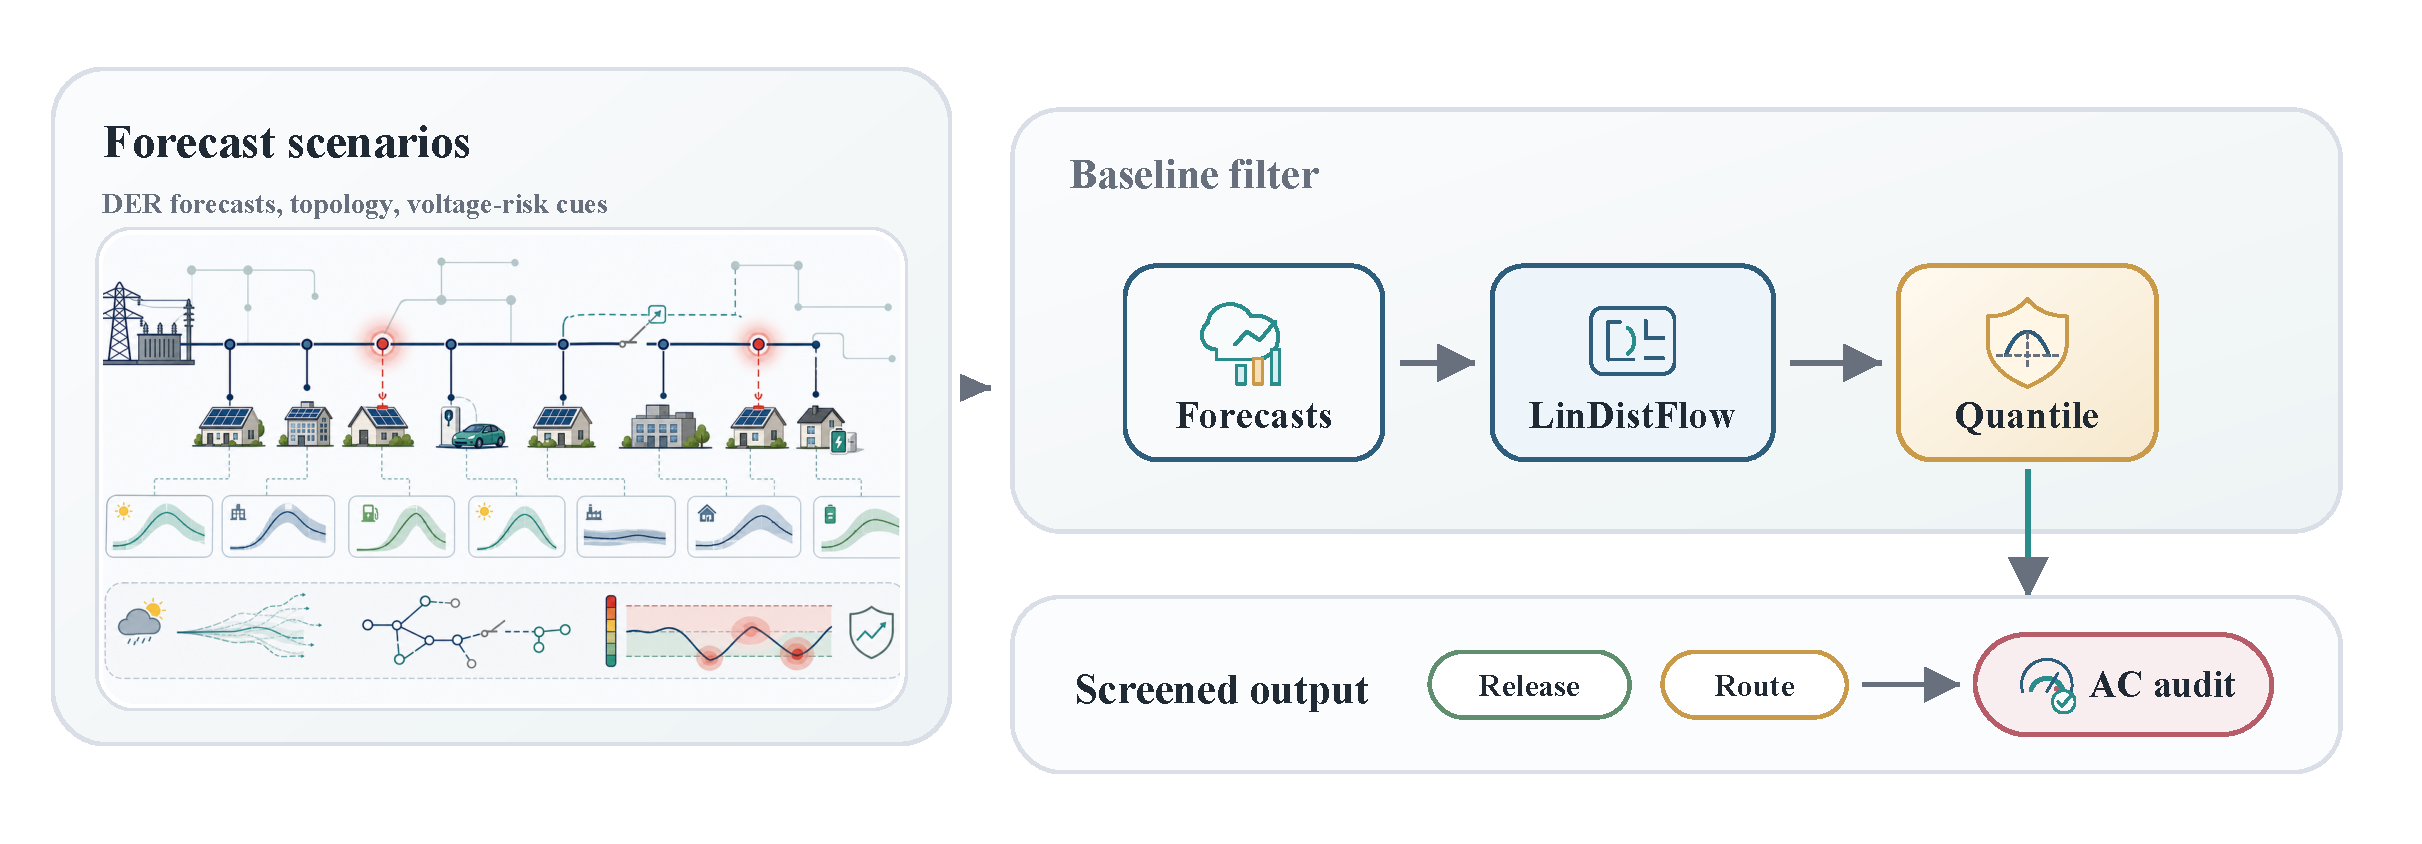
\includegraphics[width=0.94\textwidth]{figures/fig11_oajpe_lindistflow_quantile_pipeline.pdf}
\caption{LinDistFlow-Quantile baseline pipeline. The baseline note uses forecast inputs, a squared-voltage LinDistFlow proxy, and one global empirical quantile before downstream AC audit.}
\label{fig:fig11_oajpe_lindistflow_quantile_pipeline}
\end{figure*}

\section{Experimental Protocol}\label{experimental-protocol}

The baseline is evaluated on IEEE 33-bus and IEEE 69-bus distribution
feeder scenarios. Each feeder contributes AC-solvable operating
scenarios with randomized loading, PV penetration, EV demand, PV siting,
and topology variants. The random interpolation split is
scenario-disjoint with training, calibration, and test partitions. The
reported representative split uses seed 7, and the multi-seed check uses
seeds 7, 17, and 42.

The evaluation is intentionally limited to baseline behavior:

\begin{itemize}
\tightlist
\item
  LinDistFlow voltage error;
\item
  global-quantile empirical coverage and interval width;
\item
  bus-level voltage-violation recall and missed violations;
\item
  scenario-level recall and false-alarm rate.
\end{itemize}

No residual learner is fit. No calibration family is used. No AC action
or optimization claim is made.

\section{Results}\label{results}

\subsection{Representative Split}\label{representative-split}

For seed 7, the LinDistFlow-only proxy has 0.00140 p.u. RMSE. With a
90\% global empirical quantile radius, the screen obtains 0.91356
empirical bus-level coverage and 0.00474 p.u. mean interval width.
Bus-level violation recall is 0.99891, with one missed bus-level
violation. Scenario-level recall is 1.00000 in this split, and the
scenario false-alarm rate is 0.03704.

These values should be interpreted as baseline behavior, not as a tuned
screening method. The interval is intentionally global and therefore
wider than a local or conditioned error model would usually need to be.
Its value is that it is easy to implement and difficult to obscure: all
uncertainty comes from one pooled calibration radius.

\subsection{Comparison with VoltGuard}\label{comparison-with-voltguard}

A direct side-by-side comparison clarifies when the baseline is
sufficient and when learning is useful. On the same representative 33/69
random split, LinDistFlow plus one global quantile keeps scenario-level
recall at 1.00000, but it does so with an interval width of 0.00474 p.u.
VoltGuard's topology/PV/loading conditioned interval keeps bus-level
recall at 0.99891 with one missed bus-level violation while reducing the
mean interval width to 0.00043 p.u. and the false-alarm rate to 0.00058.

\begin{table*}[t]
\centering
\caption{Contextual comparison between the baseline and the VoltGuard method on the same representative random split.}
\label{tab:baseline_vs_voltguard}
\begin{tabular}{lrrrrrrr}
\hline
Screen & RMSE & Coverage & Width & Bus recall & False alarm & Missed buses & Scenario recall \\
\hline
LinDistFlow + global quantile & 0.00140 & 0.91356 & 0.00474 & 0.99891 & 0.00365 & 1 & 1.00000 \\
VoltGuard topology/PV/loading conformal & 0.00011 & 0.93660 & 0.00043 & 0.99891 & 0.00058 & 1 & 1.00000 \\
\hline
\end{tabular}
\end{table*}

This comparison does not turn the baseline note into a learned-method
paper. It shows the baseline's practical envelope. For rough triage on
small, balanced feeders, the physical-quantile screen may be sufficient.
When a workflow needs sharper intervals, fewer false alarms,
family-level calibration analysis, or topology/PV/load shift audits, the
learned residual screen becomes necessary.

\subsection{Three-Seed Check}\label{three-seed-check}

Across seeds 7, 17, and 42, the mean LinDistFlow RMSE is 0.00148 p.u.,
the mean empirical coverage is 0.91629, and the mean interval width is
0.00500 p.u. Mean scenario-level recall is 1.00000 in the tested split
family, while the mean scenario false-alarm rate is 0.05917. These
numbers show the main tradeoff of the baseline: the physical proxy plus
global quantile can preserve scenario recall in this dataset, but it
does so with a pooled radius that is not tailored to feeder, PV,
loading, or topology conditions.

\begin{figure}[t]
\centering
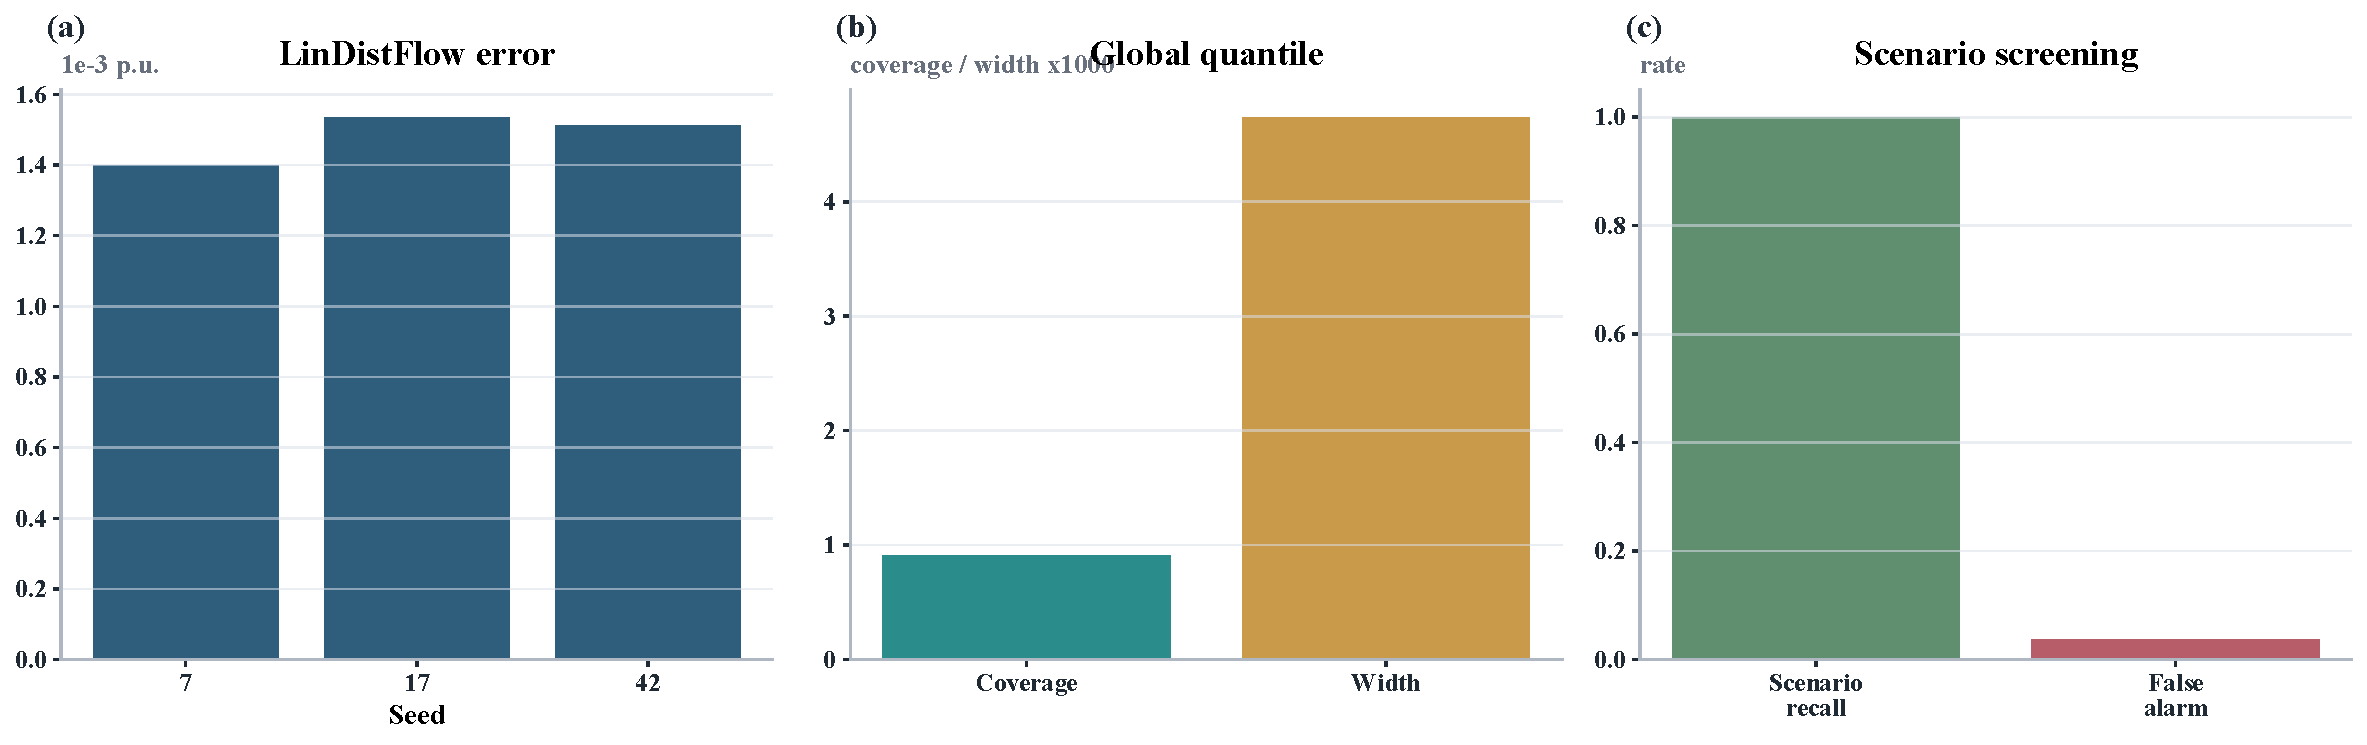
\includegraphics[width=\linewidth]{figures/fig12_oajpe_minimal_performance.pdf}
\caption{Minimal baseline performance summary. (a) LinDistFlow voltage error across seeds; (b) empirical coverage and mean interval width for the global quantile interval; (c) scenario-level screening behavior.}
\label{fig:fig12_oajpe_minimal_performance}
\end{figure}

\section{Boundary and Use}\label{boundary-and-use}

The global quantile relies on the calibration and test scenarios being
drawn from the stated scenario family. It is not a distribution-free
safety guarantee under arbitrary topology switching, arbitrary forecast
drift, unseen feeder states, or unmodeled phase imbalance. When
telemetry is stale, the topology is uncertain, the scenario lies outside
the calibration envelope, or voltage limits are already close, the
baseline should route the case to AC analysis rather than release it.

The recommended use of this note is comparative. A proposed learned,
conditioned, or optimization-aware screen should report whether it
improves over this LinDistFlow-global-quantile baseline in interval
width, missed violations, false alarms, and scenario-level behavior
under the same split protocol.

The appropriate venue is a short technical note, letters-format paper,
arXiv reference artifact, or supplement to a larger screening-method
submission. A full research-article venue should be used only if the
contribution is framed as community baseline standardization rather than
as a new screening algorithm.

Real-world validation remains outside the scope of this baseline note.
The same equations should be tested on utility or OpenDSS/SMART-DS
feeders before being treated as a deployment-ready heuristic.

\section{Conclusion}\label{conclusion}

This paper gives a small, reproducible LinDistFlow-global-quantile
baseline for distribution voltage-risk filtering. Its scientific
question is not how to build the strongest voltage-risk screen, but how
a transparent physical proxy with one pooled empirical radius behaves.
That narrow scope makes it a useful baseline implementation note and
separates it from learned residual, conditioned calibration, and DMS
integration manuscripts.

\section*{Acknowledgment}\label{acknowledgment}
\addcontentsline{toc}{section}{Acknowledgment}

The authors thank the maintainers of the open-source power-system
modeling tools and public benchmark feeders used in this study.

\section*{Funding}\label{funding}
\addcontentsline{toc}{section}{Funding}

This research did not receive any specific grant from funding agencies
in the public, commercial, or not-for-profit sectors.

\section*{Code and Data Availability}\label{code-and-data-availability}
\addcontentsline{toc}{section}{Code and Data Availability}

The experiments use publicly available IEEE test systems implemented
through pandapower and a project-local IEEE 69-bus feeder
implementation. The baseline implementation, scenario-generation
scripts, table-generation scripts, manuscript sources, and release PDFs
are publicly archived at
\texttt{https://github.com/Zhaosiqiang/voltguard-voltage-risk-screening/releases/tag/v1.0.0-submission}
and on Zenodo with DOI \texttt{10.5281/zenodo.21149702}.

\section*{Conflict of Interest}\label{conflict-of-interest}
\addcontentsline{toc}{section}{Conflict of Interest}

The authors declare that they have no known competing financial
interests or personal relationships that could have appeared to
influence the work reported in this paper.

\section*{AI Tool Use Disclosure}\label{ai-tool-use-disclosure}
\addcontentsline{toc}{section}{AI Tool Use Disclosure}

During the preparation of this work, the authors used AI-assisted coding
and language tools for drafting support, code scaffolding, consistency
checks, and language refinement. The authors reviewed and edited all
generated text and code, verified the equations and numerical claims,
and take full responsibility for the content of the article.

\section*{References}\label{references}
\addcontentsline{toc}{section}{References}

{[}1{]} Baran ME, Wu FF. Network reconfiguration in distribution systems
for loss reduction and load balancing. IEEE Transactions on Power
Delivery. 1989;4(2):1401-1407. https://doi.org/10.1109/61.25627.

{[}2{]} Farivar M, Low SH. Branch flow model: relaxations and
convexification, Part I. IEEE Transactions on Power Systems.
2013;28(3):2554-2564. https://doi.org/10.1109/TPWRS.2013.2255317.

{[}3{]} Dall'Anese E, Zhu H, Giannakis GB. Optimal power flow for
distribution networks under constraints. IEEE Transactions on Smart
Grid. 2013;4(3):1460-1471. https://doi.org/10.1109/TSG.2013.2247644.

{[}4{]} Turitsyn K, Sulc P, Backhaus S, Chertkov M. Options for control
of reactive power by distributed photovoltaic generators. Proceedings of
the IEEE. 2011;99(6):1063-1073.

{[}5{]} Robbins BA, Hadjicostis CN, Dominguez-Garcia AD. A two-stage
distributed architecture for voltage control in power distribution
systems. IEEE Transactions on Power Systems. 2013;28(2):1470-1482.

{[}6{]} Vovk V, Gammerman A, Shafer G. Algorithmic Learning in a Random
World. Springer; 2005. https://doi.org/10.1007/b106715.

{[}7{]} Shafer G, Vovk V. A tutorial on conformal prediction. Journal of
Machine Learning Research. 2008;9:371-421.

{[}8{]} Romano Y, Patterson E, Candes E. Conformalized quantile
regression. Advances in Neural Information Processing Systems. 2019;32.

{[}9{]} Angelopoulos AN, Bates S. A gentle introduction to conformal
prediction and distribution-free uncertainty quantification. Foundations
and Trends in Machine Learning. 2023;16(4):494-591.

{[}10{]} IEEE PES Distribution System Analysis Subcommittee. IEEE PES
distribution test feeders. IEEE Power \& Energy Society; accessed 2026.

{[}11{]} Thurner L, Scheidler A, Schafer F, Menke JH, Dollichon J, Meier
F, et al.~pandapower: an open-source Python tool for convenient
modeling, analysis, and optimization of electric power systems. IEEE
Transactions on Power Systems. 2018;33(6):6510-6521.

{[}12{]} Molzahn DK, Dorfler F, Sandberg H, Low SH, Chakrabarti S,
Baldick R, et al.~A survey of distributed optimization and control
algorithms for electric power systems. IEEE Transactions on Smart Grid.
2017;8(6):2941-2962. https://doi.org/10.1109/TSG.2017.2720471.

{[}13{]} Karagiannopoulos S, Aristidou P, Hug G. Data-driven local
control design for active distribution grids using off-line optimal
power flow and machine learning techniques. IEEE Transactions on Smart
Grid. 2019;10(6):6461-6471.

\end{document}
